\chapter{Aplikacja}
Uruchomiony ekosystem prezentuje logi tak jak na \refsource{schemacie}{fig:dcc}.\ Konfigurację uruchamia się za pomocą \refsource{polecenia}{lst:dcc}.

\begin{lstlisting}[language=bash, label={lst:dcc}, caption={Uruchomienie Docker Compose}]
    $ docker compose up
\end{lstlisting}

\begin{figure}[H]
    \centering
    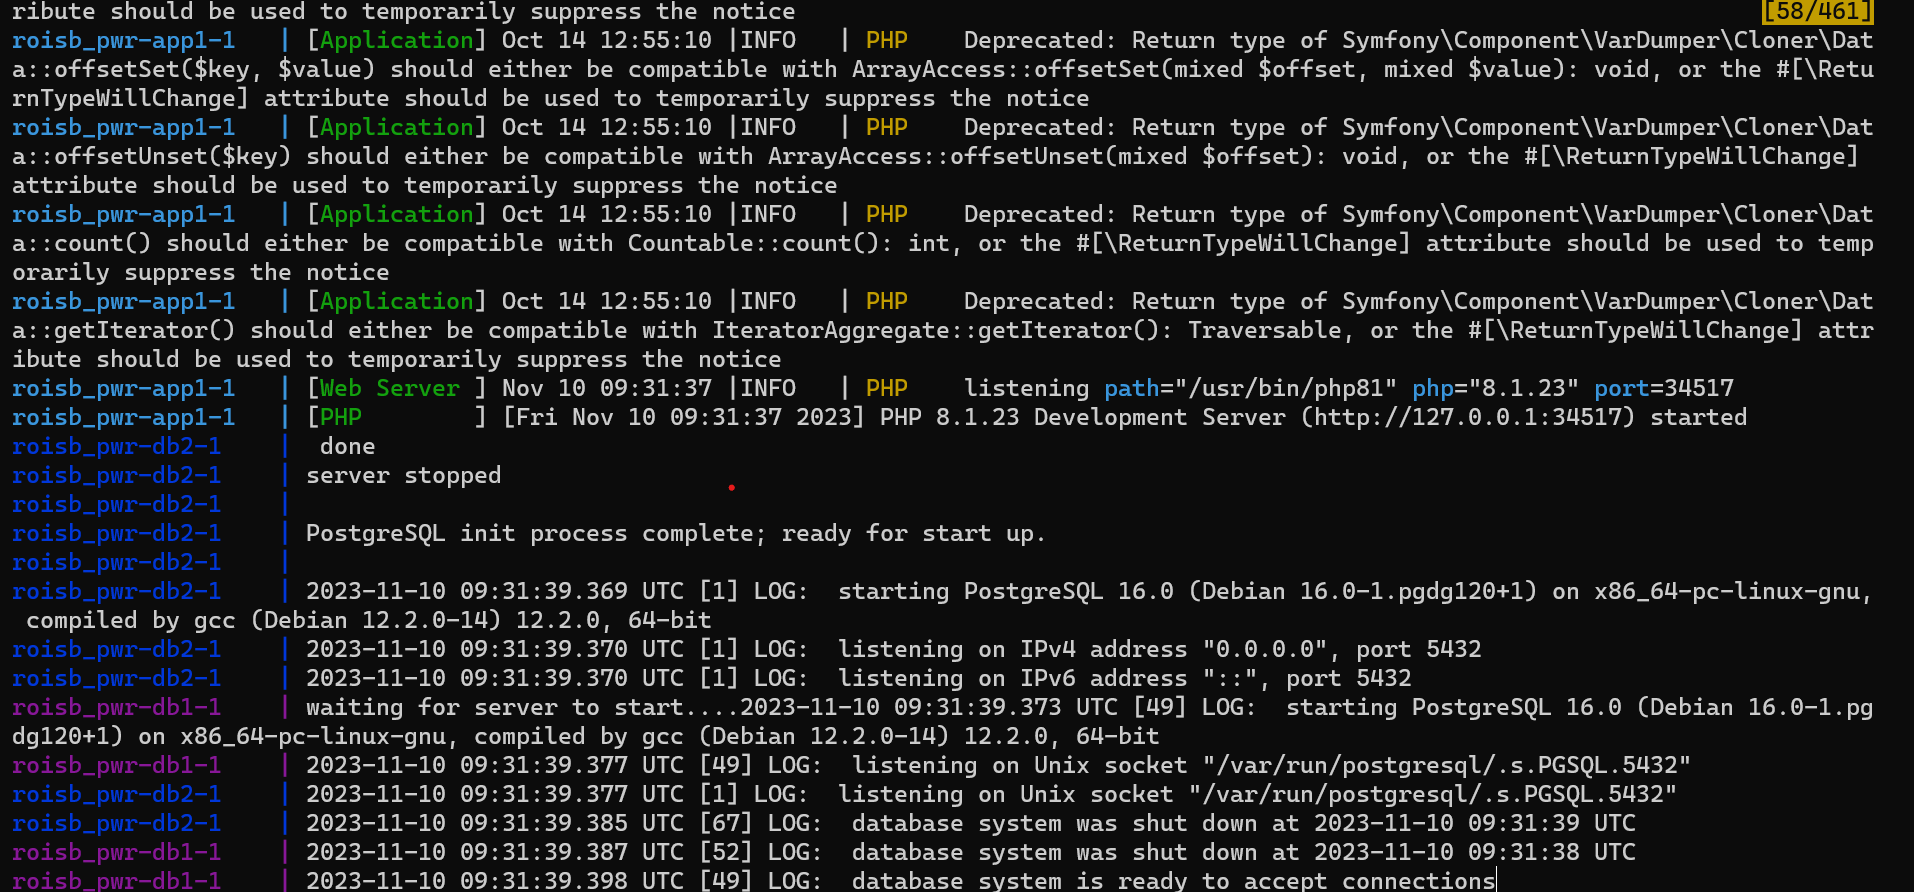
\includegraphics[width=0.7\textwidth]{images/compose}
    \captionsource{Uruchomiony Docker Compose}{Opracowanie własne}
    \label{fig:dcc}
\end{figure}

Po wprowadzeniu nowej książki do aplikacji pod adresem \textit{localhost:8081} oraz przejściu pod adres \textit{localhost:8082}, \textit{localhost:8083} można zauważyć, że zmiany wprowadzone po uruchomieniu aplikacji Bucardo, zostały rozpropagowane dalej.\ Widać to na \textbf{zdjęciach}: \textbf{\ref{fig:aa}, \ref{fig:aaa}}.

\begin{figure}[H]
    \centering
    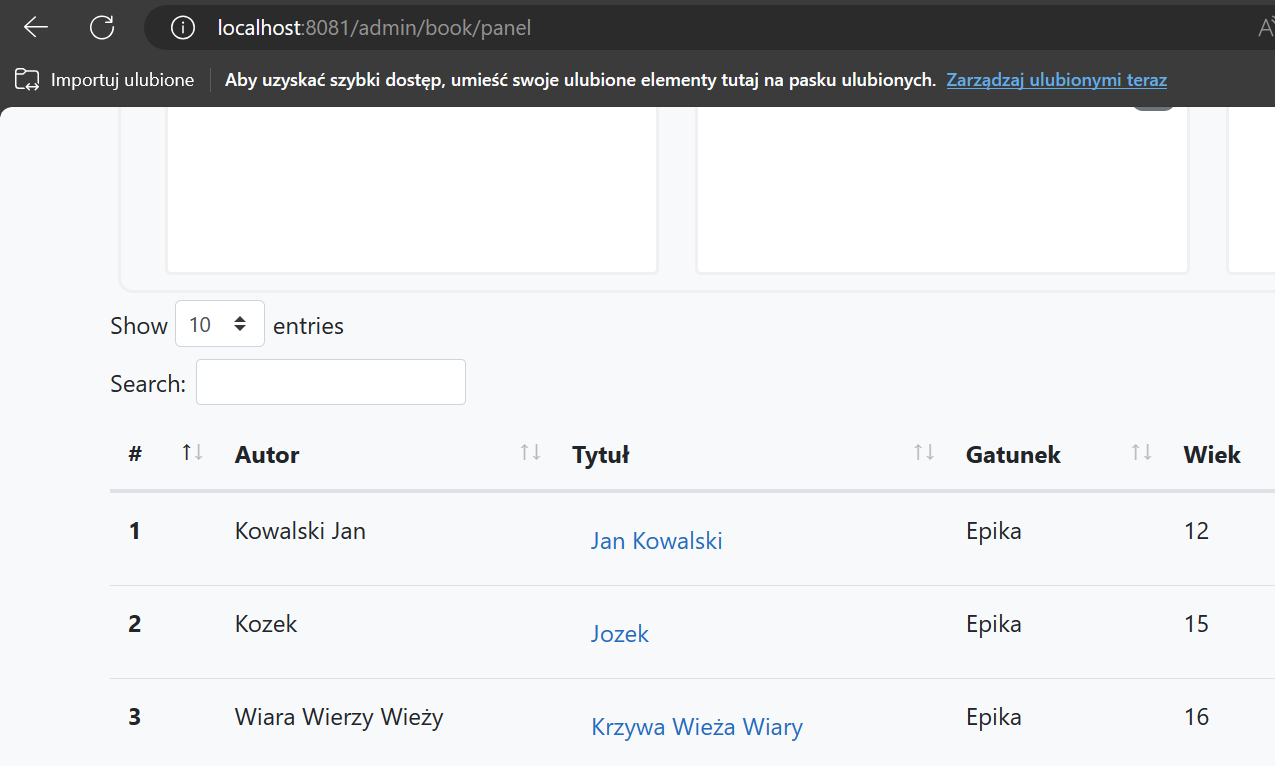
\includegraphics[width=0.5\textwidth]{images/a1}
    \captionsource{Dodanie dwóch wpisów do tabeli po uruchomieniu Bucardo}{Opracowanie własne}
    \label{fig:aa}
\end{figure}

\begin{figure}[H]
    \centering
    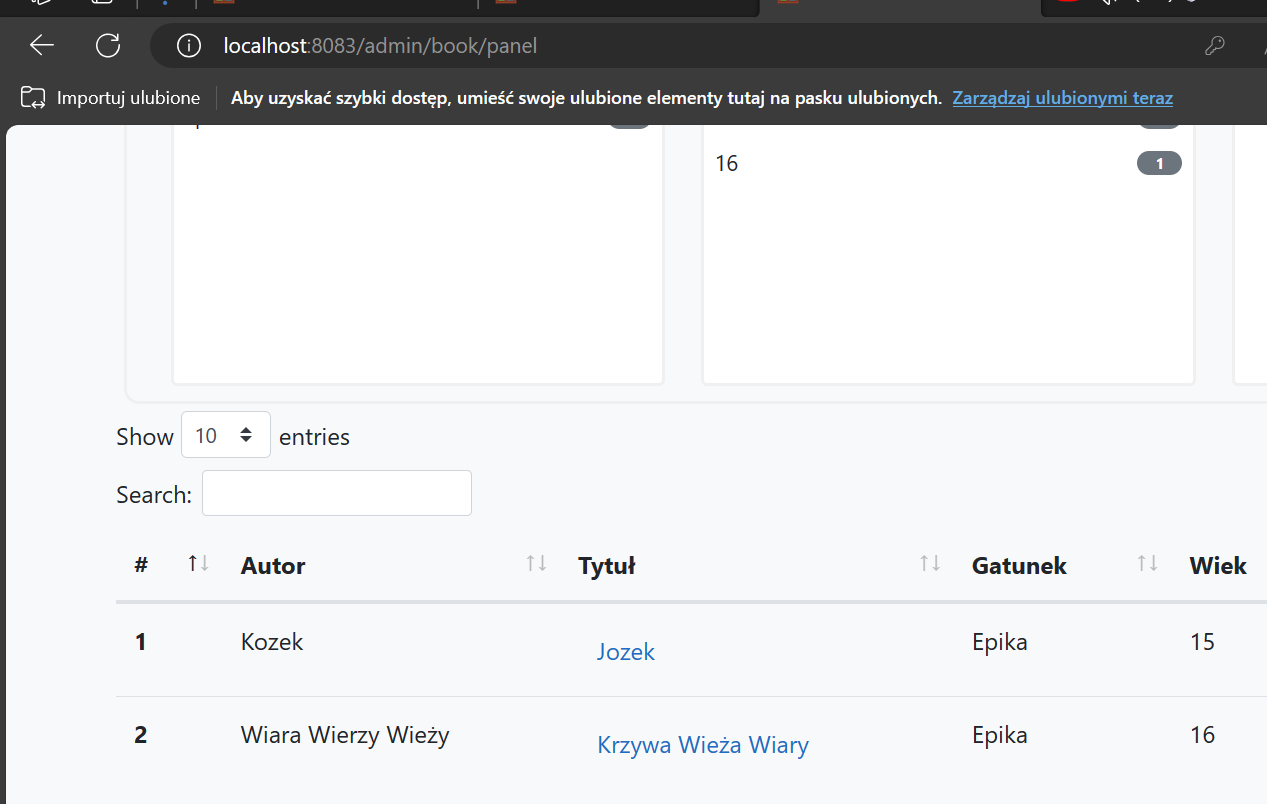
\includegraphics[width=0.5\textwidth]{images/a2}
    \captionsource{Rozpropwagowanie dwóch wpisów do tabeli po uruchomieniu Bucardo}{Opracowanie własne}
    \label{fig:aaa}
\end{figure}

\section{Podsumowanie}
Wykorzystanie replikacji baz danych pozwala na swobodne tworzenie kopii zapasowych oraz rozładowanie ruchu sieciowego.\ Pozwala to na swoistą regionalizację aplikacji, umożliwiając użytkownikom korzystanie z serwerów znajdujących się w ich regionie.\ Dodatkowo do stworzenia tego typu instancji bardzo przydatny okazał się \textit{Docker}, pozwolił on na stworzenie jednakowych obrazów aplikacji, które mogą posłużyć do uruchomienia na odpowiednim serwerze, co zostało zobrazowane a pomocą narzędzia \textit{Docker Compose}, które umożliwiło zrobienia pseudoregionalizacji, tworząc cały ekosystem aplikacji tak jak na \refsource{schemacie}{fig:roisb}.\ Wykorzystanie narzędzia \textit{Bucardo} pozwoliło na utworzenie replikacji ''\textit{master-master}'', która nie znajduje się domyślnie w bazie danych \textit{PostgreSQL}.\ Wykorzystana replikacja umożliwiła na niezależną synchronizację danych pomiędzy bazami danych.\ Synchronizacja ta dzieje się niezależnie od instancji aplikacji klienckich oraz bazy danych.\ Ponieważ \textit{Bucardo} to narzędzie reagujące na wydarzenie, w tym wypadku zmiana w bazie danych, a następnie propagujące to wydarzenie na pozostałe serwery bazodanowe.\ Aplikacja ta dzięki temu, że znajduje się na serwerze bazodanowym, wykonuje się jedynie w momencie kiedy ta baza ''\textit{działa}''.